\pagebreak
\section{Microcontrollore}
Il microcontrollore usato  è il NUCLEO H743ZI2ed è stato usato il programma dato dalla fabbrica produttrice, STM.\\
\subsection{Funzionamento generale}
Il \mu - controllore usato sfrutta la struttura interna di Harvard, ovvero con 2 memorie separate: una per i programmi e una per i dati..\\
\begin{figure}
    \centering
    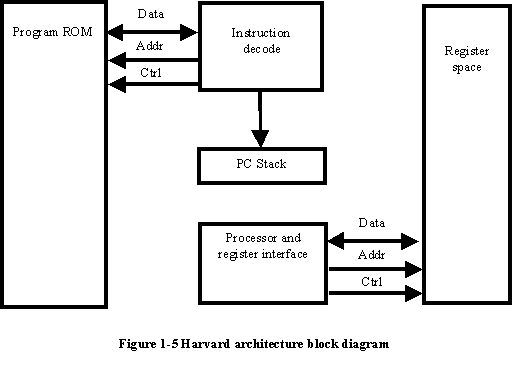
\includegraphics[width=0.5\linewidth]{assets/microcontrollore/Harvard.png}
    \caption{Struttura interna del microcontrollore}
\end{figure}
Questa struttura, unita ad un doppio bus asincrono, permette di eseguire più operazioni in parallelo, aumentando la velocità di esecuzione.


\subsection{GPIO}

\subsection{USART}

\subsection{ADC}

\subsection{DMA}

\subsection{DAC e Comparatore}